\setchapterpreamble[u]{\margintoc}
\chapter{Medina's (2007) model}
\labch{medina}

% \section{Medina's (2007) model} \labsec{medinamodel}

\textcite{Medina2007} created a Stochastic Optimality Theoretic model of the indefinite object drop. An implicit object output, generated by Gen on the basis of the input (\refsec{inputmedina}), is evaluated against a set of conflicting constraints (\refsec{constraintsmedina}). The constraints stem directly from the set of object drop predictors chosen by the author (\refsec{predictorsmedina}), and get re-ranked with respect to the verb's semantic selectivity (\refsec{rankingmedina}), computed as the Selectional Preference Strength by \textcite{Resnik1993, Resnik1996}. The way this model implements a probabilistic ranking of the constraints (detailed in \refsec{medinacomputation}) ensures not only that both implicit and overt objects are allowed in the grammar, but also that an implicit object output has a relative gradient grammaticality across different verbs.


\section{The input and the output} \labsec{inputmedina}

As I mentioned in \refsec{classicot}, Optimality Theory requires the input to syntactic optimization to contain the relevant lexical and semantic components that will be mapped to syntactically well-formed output forms. Since \textcite{Medina2007} defines a model of the indefinite object drop, her input has to provide all the information necessary to generate the two outputs in  \ref{medina_output_generic}:
% \vspace{-0.5cm} % PER AGGIUSTARE LO SPAZIO PRIMA DEGLI ESEMPI!
\ex. \label{medina_output_generic} \a. John was writing.
\b. John was writing something.

Hence, at the very least, the input will contain a transitive verb with its complete predicate-argument structure, i.e., a specified subject and an unspecified object. Since the model does not deal with \textit{specified} object drop, the input to the model cannot generate an output with a definite overt object as in \ref{medina_output_wrong}. To put it better, \textcite[70-71]{Medina2007} observes that this output may actually be in the candidate set, but it is always ruled out by a high-ranking faithfulness constraint that keeps output candidates from containing semantically richer information than in the input.
% \vspace{-0.5cm} % PER AGGIUSTARE LO SPAZIO PRIMA DEGLI ESEMPI!
\ex. \label{medina_output_wrong} John was writing a book.

In addition to this, the input will also feature all the relevant predictors of object drop used by the author, i.e., semantic selectivity (operationalized as Resnik's Selectional Preference Strength), telicity, and perfectivity. Thus, inputs in \textcite{Medina2007} have the form \ref{medina_input_generic}:
% \vspace{-0.5cm} % PER AGGIUSTARE LO SPAZIO PRIMA DEGLI ESEMPI!
\ex. \label{medina_input_generic} verb (x,y), x = subject, y = unspecified, SPS = \textit{numerical value}, [+ Past], [$\pm$ Telic], [$\pm$ Perfective]

The tense feature is fixed at [+ Past] since the author only modeled past tenses for consistency, but there is no hard theoretical constraint on this. In theory, it would indeed be possible to create similar inputs with other tenses. Looking at a specific case, the input generating the outputs in \ref{medina_output_generic} would look like \ref{medina_input_teach}.
% \vspace{-0.5cm} % PER AGGIUSTARE LO SPAZIO PRIMA DEGLI ESEMPI!
\ex. \label{medina_input_teach} write (x,y), x = John, y = unspecified, SPS = 2.54\sidenote{This is the value of Selectional Preference Strength that Resnik obtained by performing the computation over the Brown corpus of English \parencite[150]{Resnik1996}, also reported in \textcite[114]{Medina2007}.}, [+ Past], [-Telic], [- Perfective]

Let us take a closer look at how the three predictors chosen by Medina are implemented in her model.

%  È GIUSTO CHE QUI GLI OGGETTI SIANO INDEFINITI!!! NELL'ESPERIMENTO SONO OVERT PERCHÈ NON RIENTRANO NEL MODELLO OT!!! 83 pdf Medina

\section{Predictors} \labsec{predictorsmedina}

\subsection{Semantic selectivity} \labsec{predmedina_semsel}

\textcite{Medina2007} uses semantic selectivity as a measure of the recoverability of a transitive verb's direct objects, which the reader will remember being a major determiner of object drop based on the information discussed in \refsec{recoverability}. As a quick recap, I will just note that the recoverability of a direct object (or, better, of the broad semantic class it belongs to) of a verb correlates with the grammaticality of sentences featuring that same verb used intransitively, as in \ref{recap_sps}.
% \vspace{-0.5cm} % PER AGGIUSTARE LO SPAZIO PRIMA DEGLI ESEMPI!
\ex. \label{recap_sps} \a. John ate $\varnothing$\textsubscript{dObj}. \\ $\longrightarrow$ The omitted object belongs to the category of Edibles.
\b. *John made $\varnothing$\textsubscript{dObj}. \\ $\longrightarrow$ The omitted object can be virtually anything.

In theory, it would be possible to treat the semantic selectivity of a transitive verb with respect to its direct objects as a binary feature and be done with it. However, this choice would be quite poor both from a methodological point of view, since there is no clear-cut criterion to tell apart recoverable-object and non-recoverable-object verbs, and from a usability point of view, since binary selectivity would be scarcely informative with respect to object drop, semantic recoverability being a gradient notion.\\
Making use of the experimental literature on the matter, \textcite{Medina2007} decided to operationalize semantic selectivity using the Selectional Preference Strength measure developed by \textcite{Resnik1993, Resnik1996}. Resnik quantifies the selectional preferences of transitive verbs in an information-theoretical model which encodes semantic selectivity as the relative entropy between the distribution of WordNet \parencite{beckwith1991wordnet, Miller1995} classes for all the direct objects in a corpus and the distribution of WordNet classes for the direct objects of a specific verb. I will discuss the mathematical meaning and the computational details of Resnik's Selectional Preference Strength in \refsec{predictor_sps}, where I will also present an update of his measure I contributed to create \parencite{CappelliLenciPISA}, powered by distributional semantics and word embeddings.\\
Here, I will only point out how suitable Resnik's measure is for the purposes of Medina's model of indefinite object drop. First of all, the Selectional Preference Strength score assigned to a verb is a numerical value (a non-null positive real number) on a continuous scale, which it makes it perfect to capture the fact that semantic selectivity is not a binary variable. In particular, the narrower the selectional preferences of a verb are (i.e., the more recoverable its direct objects are), the greater the Selectional Preference Strength of that verb is. Most conveniently for Medina's thesis in acquisitional linguistics, whose scope goes far beyond the coding of computational technicalities, \textcite[150]{Resnik1996} provides the Selectional Preference Strength scores computed for 34 English verbs over the Brown corpus \parencite{kucera1967brownCorpus}, the CHILDES corpus \parencite{macwhinney2000childesCorpus}, and human subject norms. While being a limited set of data, this collection of scores has all the data Medina needed to build her model of the implicit object construction, and it is still a valuable resource for anyone looking into models of semantic selectivity.


\subsection{Telicity} \labsec{medinatelicity}
Telicity has been proven to be an important predictor of the omissibility of direct objects in \refsec{telicity}. Medina encodes it as a binary variable, so that the transitive verbs she tested (Resnik's 34 ones) are tagged as either telic or atelic. Doing so, however, is less straightforward than it may seem at first glance.\\
Telicity, in its typical interpretation, is a property of predicates, in conjunction with their grid of arguments and the way they are filled by linguistic material \parencite{Vendler1957, dowty2012word1979}. This means that the (a)telicity feature may only be assigned to complete verb phrases, complete with arguments and adjuncts, and not to bare verb heads (see the simplified tree in \reffig{telicity_at_vp_tree}). Under this view, predicates are telic if the events they describe have an endpoint (encoded as a direct object), or they are atelic if they don't. As a logical consequence, the same verb would be considered telic when used transitively and atelic when used intransitively \parencite{OlsenResnik1997, Mittwoch1982}.

\begin{figure}[htb]
\caption{Simplified syntax tree illustrating the traditional interpretation of telicity as a property of predicates, not verb heads.}
\labfig{telicity_at_vp_tree}
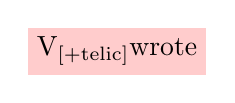
\begin{tikzpicture}
\Tree [.TP [.DP \edge[roof]; {John} ] [.T' [. \node(x){T\\$\varnothing$\textsubscript{[+past]}}; ] [.\node[fill=green!20] {VP\textsubscript{[+telic]} };[.V' [.\node[fill=red!20] {V\textsubscript{\sout{[+telic]}}\\wrote}; ] [.DP \edge[roof]; {a book} ] ] ] ] ]
% \draw[semithick, <-] (x) to [bend right=70] (y);
\end{tikzpicture}
\end{figure}

As Medina points out, telicity taking scope over a whole verb phrase poses a severe problem with respect to the use of telicity as a predictor of object drop. How can an object-dropping transitive verb be always considered (a)telic, if the very act of adding or dropping its object alters its telicity? Medina's solution to this conundrum makes use of the analysis of telicity as a privative feature by \textcite{Olsen1997}. Let us discuss this approach in more detail.\\
According to \textcite[32]{Olsen1997}, telicity is a semantic feature verbs have if the event they denote can have an endpoint or a result, regardless of whether they actually attain it or not. Based on this, [+telic] verbs cannot lose the feature even if the endpoint is not realized as a syntactic constituent. On the contrary, atelicity is a cancelable conversational implicature, so [-telic] verbs can be interpreted as either having or not having an inherent endpoint or result. To prove this point, Olsen provides two series of examples (adapted from \textcite[33]{Olsen1997}), reported in \ref{telic_intro} and \ref{atelic_intro}. In \ref{telic_intro}, telicity is shown to be an inherent semantic property with a non-cancelable marked interpretation, since the addition of the durative adverbial 'for years' turns the accomplishments into \textit{iterative} accomplishments, not into activities (which are [-telic], [+durative] predicates).

\ex. \label{telic_intro} \a. \label{telic_intro1} Eli won for years.
\b. \label{telic_intro2}  Eli ran to the store for years.

Instead, examples in \ref{atelic_intro} demonstrate the unmarked nature of atelicity, based on the assumption that progressive forms of atelic verbs entail the corresponding perfect form (as in \ref{atelic_intro2}), while the same is not true of telic verbs (as in \ref{atelic_intro1} and \ref{atelic_intro3}). Thus, it is possible to add material and disrupt the atelic interpretation (compare \ref{atelic_intro2} with \ref{atelic_intro3}), but it is not possible to cancel telicity (as shown in \ref{telic_intro1} and \ref{telic_intro2}).

\ex. \label{atelic_intro} \a. \label{atelic_intro1} Eli is winning. $\nsucc$ Eli has won.
\b. \label{atelic_intro2}  Eli is running. $\succ$ Eli has run.
\c. \label{atelic_intro3}  Eli is running to the store. $\nsucc$ Eli has run to the store.

Olsen (followed by Medina) actually uses the notation [0 Telic] to indicate the feature of verbs which lack telic denotation, but in this thesis I will use a more transparent opposition between [+telic] and [-telic] verbs. Now informed about the underlying theory (discussed in more detail in \refsec{telicity}), the reader will be able to interpret the [-telic] feature as Olsen intended.\\
By virtue of this particular interpretation of telicity, Medina considers verbs such as \textit{to make} to be [+telic] and verbs such as \textit{to eat} to be [-telic]. The author assigns telicity (or lack thereof) to each verb on the basis of three tests\sidenote{All the examples in the list are taken \textit{verbatim} from \textcite[302-303]{Medina2007}.}.

\begin{itemize}
    \item \textbf{The \textit{in/for} test} \parencite{dowty2012word1979, Vendler1957}. Predicates featuring [+telic] verbs, as in \ref{telicitytest_infor1}, allow more easily \textit{in-X-time} temporal adverbs and less easily \textit{for-X-time} temporal adverbs, while predicates with [-telic] verbs, as in \ref{telicitytest_infor2}, have the reverse preference pattern.
    
\ex. \label{telicitytest_infor} \a. \label{telicitytest_infor1} Michelle made some stuff in/*for five minutes.
\b. \label{telicitytest_infor2}  Michelle read *in/for five minutes.
    
    \item \textbf{The \textit{almost} test} \parencite{dowty2012word1979}. The adverb \textit{almost} allows [+telic] verbs, as in \ref{telicitytest_almost1}, to have two interpretations (the event has begun but has not finished yet; the event has not begun yet), while [-telic] verbs, as in \ref{telicitytest_almost2}, can have only one (the event has not begun yet).
    
\ex. \label{telicitytest_almost} \a. \label{telicitytest_almost1} Tony almost packed.\\ $\longrightarrow$  Tony started packing, but hasn’t finished yet. \\ $\longrightarrow$  Tony was about to pack but hadn’t yet started.
\b. \label{telicitytest_almost2} Tony almost ate.\\ $\longrightarrow$  \sout{Tony started eating, but hasn’t finished yet.} \\ $\longrightarrow$  Tony was about to eat but hadn’t yet started.
    
    \item \textbf{The \textit{counting} test} \parencite{bach1986algebra}. It is more acceptable to count [+telic] predicates, as in \ref{telicitytest_counting1}, than [-telic] ones, as in \ref{telicitytest_counting2}. In other words, counted [+telic] predicates are interpreted as a single event with repeated acts, while counted [-telic] predicates are interpreted as repeated, distinct events. This is the most controversial test out of the three Medina chose to use.

\ex. \label{telicitytest_counting} \a. \label{telicitytest_counting1} Edgar opened some stuff three times.
\b. \label{telicitytest_counting2}  Edgar watched three times.

\end{itemize}

Medina tested her target verbs in combination with an indefinite object or in an intransitive sentence. A transitive verb tested this way is [+telic] if at least two tests out of three yield a telic interpretation or [-telic] otherwise, based on the assumption that the verb lacks telic denotation (i.e., is atelic) if it can elicit both a telic and an atelic interpretation. As I will discuss in more detail in \refsec{predictor_telicity}, while the \textit{in/for} test is a largely reliable diagnostic for telicity, the other two tests are somewhat problematic.


\subsection{Perfectivity} While telicity (i.e., lexical aspect) is a semantic property of individual verbs, as illustrated in the previous paragraph, perfectivity (i.e., grammatical aspect) in English is morphologically marked. A more detailed discussion of the effects of perfectivity on the grammaticality of indefinite object drop is provided in \refsec{perfectivity}.\\
As noted in \refsec{inputmedina}, \textcite{Medina2007} only modeled inputs in the past tense. With respect to the morphological markers of (im)perfectivity, the author followed \textcite{Olsen1997} in realizing [+perfective] inputs with perfect morphology, in the form "\textit{have} + past participle of the verb", as in \ref{medina_perfectivity1}, and [-perfective] inputs with progressive morphology, in the form "\textit{be} + verb + \textit{-ing}", as in \ref{medina_perfectivity2}.

\ex. \label{medina_perfectivity} \a. \label{medina_perfectivity1} John had written a book.
\b. \label{medina_perfectivity2}  John was writing a book.

In my own models of object drop (presented in \nrefch{model}), I marked (im)perfective aspect on English verbs using the same morphology as in \textcite{Medina2007}, and I devised a similar strategy for my Italian stimuli (\refsec{predictor_perfectivity}).


\section{Constraints and their ranking} \labsec{constraintsmedina}

For each input to the optimization in Medina's model, the two candidate outputs (one with an overt object, one with an implicit object, as detailed in \refsec{inputmedina}) are evaluated against the four constraints in \ref{medina_constraints}. Their labels and definitions are taken \textit{verbatim} from \textcite[72]{Medina2007}.

% A set of four candidates is being evaluated against the same one markedness and three faithfulness constraints

\ex. \label{medina_constraints} 
\a. \label{medina_constraints_intarg} \textsc{*Int Arg (*Internal Argument Structure)}\\ The output must not contain an overt internal argument (that is to say, a direct object).
\b. \label{medina_constraints_faith} \textsc{Faith Arg (Faithfulness to Argument Structure)}\\ All arguments in the input must be present in the output.
\c. \label{medina_constraints_telic} \textsc{Telic End (Telic Endpoint)}\\ The endpoint of a [+ Telic] event must be bounded by the presence of an overt argument in the output.
\c. \label{medina_constraints_perf} \textsc{Perf Coda (Perfective Coda)}\\ The coda of a perfective event [+ Perfective] must be identified by the presence of an overt argument in the output.

Let us discuss each constraint more extensively. \textsc{*Int Arg\sidenote{In Optimality Theory, constraints are named after features or linguistic elements required in the grammar. An asterisk is added at the beginning of a constraint's name if that constraint is violated by the presence, not the absence, of a particular feature.}} is a markedness constraint belonging to a broader class of economy-of-structure constraints, \textsc{*Struc} \parencite{buchwald2002recoverability, hartkemeyer2000ot}, operating in syntax and every other domain of grammar. By penalizing candidates with an overt object, which have a greater degree of syntactic structure than candidates with an implicit object, \textsc{*Int Arg} is the only constraint in Medina's set to favor implicit-object candidates. As I will explain in \refsec{rankingmedina}, this unique behavior of \textsc{*Int Arg} is not just intended, but downright necessary for the probabilistic re-ranking of the constraint to happen.\\
\textsc{Faith Arg} is a faithfulness constraint requiring that all arguments in the input be overtly realized in the output, thus penalizing candidates with an implicit object. As discussed in \refsec{classicot}, faithfulness constraints are a unique feature of Optimality Theory, created in order to conflict with economy-of-structure markedness constraints like the framework requires. Without faithfulness constraints, the optimal candidate would always be the least marked one, i.e., the one violating the lowest-ranked constraints \parencite[3]{legendre2001introduction}. In the specific case of Medina's model, \textsc{Faith Arg} conflicts directly with \textsc{*Int Arg}, determining a state of affairs that closely resembles the situation previously described in \reffig{stochot_gaussians_dobj}. The picture is made more complex by the interaction of two additional constraints and the inclusion of semantic selectivity in the model.\\
Finally, the markedness constraints \textsc{Telic End} and \textsc{Perf Coda} are the Optimality Theoretic implementations of telicity (\refsec{telicity}) and perfectivity (\refsec{perfectivity}) as predictors of object drop, both penalizing object-dropping output candidates. Notably, while \textsc{*Int Arg} and \textsc{Faith Arg} are always active regardless of the input features, \textsc{Telic End} and \textsc{Perf Coda} are only actively used by the \textsc{Eval} component if the input is, respectively, [+telic] and [+perfective]. Let us consider the examples in \reftab{medina2007_Ytel_Yperf} to \reftab{medina2007_Ntel_Nperf}, adapted from \textcite{Medina2007}. The absence of the pointing hand indicates that no winner has been chosen among the candidates, since these examples are just here to illustrate the possible violation profiles determined by different inputs. In the same spirit, the dotted lines show that no constraint ranking (neither in standard nor in stochastic Optimality Theory) has been determined.\\
A transitive verb which is both telic and perfective, such as \textit{to catch} in \reftab{medina2007_Ytel_Yperf}, has a full constraint violation profile involving all the four constraints at play in Medina's model. Instead, the output candidates for a telic but imperfective input verb (such as \textit{to catch} in \reftab{medina2007_Ytel_Nperf}) only violate \textsc{*Int Arg}, \textsc{Faith Arg}, and \textsc{Telic End}. In this situation, \textsc{Perf Coda} is vacuously satisfied, i.e., there is no candidate in the candidate set with the ability to violate the constraint (given that it is violated by object-dropping perfective candidates, and here there is none). Similarly, \textsc{Telic End} is vacuously satisfied in \reftab{medina2007_Ntel_Yperf}, and both \textsc{Telic End} and \textsc{Perf Coda} are vacuously satisfied in \reftab{medina2007_Ntel_Nperf}. In these four tableaux, vacuously satisfied constraints are marked in light gray for the sake of clarity. Typically, authors leave them out of their tableaux in Optimality Theoretic literature.

\begin{table}[htb] % the "htb" makes table env unfloaty
\caption{Optimality Theory tableau illustrating the constraint violation profile in the model of object drop by \textcite{Medina2007}, relative to a telic perfective verb.}
\labtab{medina2007_Ytel_Yperf} % \hand a.
\begin{adjustbox}{max width=\textwidth}
\begin{tabular}{|ll||c;{1pt/1pt}c;{1pt/1pt}c;{1pt/1pt}c|}\hline   
      & \vtop{\hbox{\strut catch (x,y), x = Jack, y = unspecified, SPS = n/a, }\hbox{\strut [+Past], [+Telic], [+Perfective]}}  & \textsc{\rotatebox[origin=c]{90}{ *Int Arg }}  &  \textsc{\rotatebox[origin=c]{90}{ Faith Arg }} & \textsc{\rotatebox[origin=c]{90}{ Telic End }} &
      \textsc{\rotatebox[origin=c]{90}{ Perf Coda }}\\
      \hline\hline
a. & Jack had caught.     &   &  *   & * & *\\ \hline
b. & Jack had caught something.     & *  &   &  & \\ \hline
\end{tabular}
\end{adjustbox}
\end{table}

\begin{table}[htb] % the "htb" makes table env unfloaty
\caption{Optimality Theory tableau illustrating the constraint violation profile in the model of object drop by \textcite{Medina2007}, relative to a telic imperfective verb.}
\labtab{medina2007_Ytel_Nperf} % \hand a.
\begin{adjustbox}{max width=\textwidth}
\begin{tabular}{|ll||c;{1pt/1pt}c;{1pt/1pt}c;{1pt/1pt}c|}\hline   
      & \vtop{\hbox{\strut catch (x,y), x = Jack, y = unspecified, SPS = n/a, }\hbox{\strut [+Past], [+Telic], [-Perfective]}}  & \textsc{\rotatebox[origin=c]{90}{ *Int Arg }}  &  \textsc{\rotatebox[origin=c]{90}{ Faith Arg }} & \textsc{\rotatebox[origin=c]{90}{ Telic End }} &
      \textsc{\rotatebox[origin=c]{90}{ \textcolor{gray}{Perf Coda} }}\\
      \hline\hline
a. & Jack was catching.     &   &  *   & * & \\ \hline
b. & Jack was catching something.     & *  &   &  & \\ \hline
\end{tabular}
\end{adjustbox}
\end{table}

\begin{table}[htb] % the "htb" makes table env unfloaty
\caption{Optimality Theory tableau illustrating the constraint violation profile in the model of object drop by \textcite{Medina2007}, relative to an atelic perfective verb.}
\labtab{medina2007_Ntel_Yperf} % \hand a.
\begin{adjustbox}{max width=\textwidth}
\begin{tabular}{|ll||c;{1pt/1pt}c;{1pt/1pt}c;{1pt/1pt}c|}\hline   
      & \vtop{\hbox{\strut eat (x,y), x = Jack, y = unspecified, SPS = n/a, }\hbox{\strut [+Past], [-Telic], [+Perfective]}}  & \textsc{\rotatebox[origin=c]{90}{ *Int Arg }}  &  \textsc{\rotatebox[origin=c]{90}{ Faith Arg }} & \textsc{\rotatebox[origin=c]{90}{ \textcolor{gray}{Telic End} }} &
      \textsc{\rotatebox[origin=c]{90}{ Perf Coda }}\\
      \hline\hline
a. & Jack had eaten.     &   &  *   &  & *\\ \hline
b. & Jack had eaten something.     & *  &   &  & \\ \hline
\end{tabular}
\end{adjustbox}
\end{table}

\begin{table}[H] % the "htb" makes table env unfloaty
\caption{Optimality Theory tableau illustrating the constraint violation profile in the model of object drop by \textcite{Medina2007}, relative to an atelic imperfective verb.}
\labtab{medina2007_Ntel_Nperf} % \hand a.
\begin{adjustbox}{max width=\textwidth}
\begin{tabular}{|ll||c;{1pt/1pt}c;{1pt/1pt}c;{1pt/1pt}c|}\hline   
      & \vtop{\hbox{\strut eat (x,y), x = Jack, y = unspecified, SPS = n/a, }\hbox{\strut [+Past], [-Telic], [-Perfective]}}  & \textsc{\rotatebox[origin=c]{90}{ *Int Arg }}  &  \textsc{\rotatebox[origin=c]{90}{ Faith Arg }} & \textsc{\rotatebox[origin=c]{90}{ \textcolor{gray}{Telic End} }} &
      \textsc{\rotatebox[origin=c]{90}{ \textcolor{gray}{Perf Coda} }}\\
      \hline\hline
a. & Jack was eating.     &   &  *   &  & \\ \hline
b. & Jack was eating something.     & *  &   &  & \\ \hline
\end{tabular}
\end{adjustbox}
\end{table}

So far, so good. However, the attentive reader will have noticed that no mention has been made of object recoverability (quantified via semantic selectivity) among the constraints at play, even though it has been said to be a crucial predictor of object drop in \refsec{recoverability} and in \refsec{predictorsmedina}. As \textcite[76]{Medina2007} observes, it would indeed be easy to define an \textsc{*Overt Recoverable Object} constraint penalizing overt objects occurring with high-selectivity verbs, or a \textsc{*Non-recoverable Implicit Object} constraint penalizing implicit objects occurring with low-selectivity verbs. This works perfectly for binary predictors such as telicity and perfectivity, but semantic selectivity is not a binary predictor (as noted in \refsec{predmedina_semsel}). Not only is it quantified by means of a continuous numerical variable, but it is structurally impossible to define a threshold value separating high- and low-selectivity transitive verbs.\\
\textcite[75]{yankes2021objectdropot} tried to account for the effect of object recoverability\sidenote{Which he calls "object subcategorization", making imprecise use of a syntactic term (referring to the number and types of syntactic arguments a verb takes) to refer to a semantic notion (the inferability of the referent of an omitted object from the semantics of the verb alone).} by introducing the faithfulness constraint (penalizing object-dropping candidates) in \ref{yankes-info}. However, Yankes merely states that a candidate violates \textsc{Info} if the verb in the input lacks recoverability "in sufficient degree", without attempting a more rigorous definition or quantification of such a degree beyond personal intuition. The blurry definition of this binary constraint is the only way to make his standard Optimality Theoretic model of indefinite null objects work, but this phenomenon has to be accounted for within a gradience-compatible framework (as argued in \refsec{ot_bad_dobjdrop}).

\ex. \label{yankes-info} \textsc{Info(rm)}: Important, noninferable speech content may not be omitted.

Let us go back to Medina's model, and her implementation of recoverability via Resnik's measure of semantic selectivity. In the original works about a computational model of semantic selectivity as a proxy to argument recoverability \parencite{Resnik1993, Resnik1996}, the author himself observed that albeit his Selectional Preference Strength measure correlates well with the acceptability of implicit objects, there are indeed some cases where a high-SPS verb does not allow for its object to be dropped (e.g., \textit{to hang, to wear}). For this reason, as I will detail in \refsec{rankingmedina}, SPS will play a crucial role in Medina's probabilistic constraint ranking, despite not being defined as a constraint \textit{per se}.\\
The gradient nature of object recoverability, be it computed via SPS \parencite{Resnik1993, Resnik1996} or measures such as PISA \parencite{CappelliLenciPISA}, makes it a bad candidate for constraint-hood. Moreover, even if it were possible to binarize it into a viable constraint, it would still suffer from a problem afflicting all the binary constraints at play, i.e., out-of-range output generation both within-constraint and across constraints. In other words, each constraint in the model under- or over-generates outputs across verbs, since experimental data show that some telic verbs occur with implicit objects while others do not, that perfective aspect favors implicit objects but does not force them, and so on. This is normal, expected behavior for classic Optimality Theoretic constraints, easily solved by means of re-ranking in order to select the winner candidate. However, in this case the state of affairs is more complicated.\\
As shown in \reftab{medina2007_Ytel_Yperf} to \reftab{medina2007_Ntel_Nperf}, forcing the implicit object construction into a standard Optimality Theoretic model (as attempted by \textcite{yankes2021objectdropot}) has two major drawbacks. One is that the same constraint violations apply to any verb with a given aspectual profile, meaning that a tableau like \reftab{medina2007_Ntel_Yperf} would apply to \textit{to eat} and to any other atelic perfective input (since, in standard Optimality Theory, the ranking of the constraints has to be consistent within the same language). As just observed, this does not match the actual linguistic data on indefinite object drop. The second issue with such a model is that it only allows for a single winner out of a candidate set, so that (also considering the previous problem) for a given aspectual profile, regardless of the specific verb in the input, the direct object would be either obligatory, or obligatorily dropped. Looking again at tableaux \reftab{medina2007_Ytel_Yperf} to \reftab{medina2007_Ntel_Nperf}, the model would determine which of the two candidates would win the competition solely based on the relative ranking of \textsc{*Int Arg} with respect to any of the other constraints (since the relative ranking of \textsc{Faith Arg}, \textsc{Telic End}, and \textsc{Perf Coda} is irrelevant for the purposes of electing a winner). Given that the the felicity of the implicit object construction depends on the interaction of several factors, and given that no factor or combination of factors actively forces or prohibits object drop, the logical conclusion is that a standard Optimality Theoretic model of object drop fails to meet the speaker's intuitions.\\
Taking all of this into consideration, a non-standard Optimality Theoretic comprehensive model of the implicit object construction based on the linguistic factors hereby described has to account for two aspects, i.e.,
\begin{enumerate}
    \item incorporating semantic selectivity (a continuous, non-binary factor) into the model, and
    \item allowing the model to yield outputs with varying degrees of grammaticality, instead of having a winner and a loser.
\end{enumerate}

\section{Defining a probabilistic constraint ranking} \labsec{rankingmedina}

\subsection{Introduction}

\textcite{Medina2007} built such a model under the premises of Stochastic Optimality Theory, whose tenets were introduced in \refsec{stochot}. This framework accounts for gradient grammaticality out-of-the-box, since it assigns each candidate a probability of it being the winner, to be interpreted as a degree of grammaticality. As for the implementation of semantic selectivity as a continuous factor, Medina came up with a personal variation on Stochastic Optimality Theory.\\
As noted in tableaux \reftab{medina2007_Ytel_Yperf} to \reftab{medina2007_Ntel_Nperf}, the winner in a Standard Optimality Theoretic model is determined based on the ranking of \textsc{*Int Arg} relative to the other three constraints at play. The same would hold true for a traditional Stochastic Optimality Theoretic version of the same model, where all constraints would be assigned a given normal distribution with a fixed evaluation noise (fully described by its standard deviation). Medina's stochastic model obtains the probability of \textsc{*Int Arg} dominating the other three constraints as a function of the verb's semantic selectivity, computed using Resnik's Selectional Preference Strength \parencite{Resnik1993,Resnik1996}. Compared with traditional Stochastic Optimality Theory, Medina's proposal achieves the same goal of having candidates with \textit{gradient} grammaticality (instead of a single absolute winner), while having two advantages:
\begin{itemize}
    \item implementing semantic selectivity in the model properly, and
    \item defining the relative ranking of \textsc{*Int Arg} with respect to the other three constraints as independent computations, yielding fine-grained interactions of semantic selectivity with telicity, perfectivity, and faithfulness to the input.
\end{itemize}
In such a model, the grammaticality of candidates is assessed across all possible constraint re-rankings, each of which is assigned a probability by the model. Medina's implementation of this model stems from a three-step logic: \labpage{3steplogicmedina}
\begin{enumerate}
    \item the probability of \textsc{*Int Arg} dominating each of the other constraints is expressed as a function of the input verb's semantic selectivity, computed via Resnik's Selectional Preference Strength;
    \item the values of the function are used to compute the relative probabilities of each of the four possible re-rankings of \textsc{*Int Arg} with respect to the three other constraints at play;
    \item these relative probabilities determine the relative probability (and thus grammaticality) of the implicit object output for a given input, depending on semantic selectivity and the input's aspectual type.
\end{enumerate}

In the next Sections, I will explain each step in depth and unveil the underlying mathematical processes. Before doing this, a brief introduction to the mathematical premises of Medina's model is in order.\\
Let us consider a hypothetical model with $n$ constraints. These constraints could be re-ranked in $n!$\sidenote{This notation stands for "n factorial" and it is equivalent to the number of possible permutations of the set ${1,2,...,n}$, i.e., a list of $n$ unique elements. It is computed as $n \cdot (n-1) \cdot (n-2) \cdot ... \cdot 1$.} ways. However, since in the stochastic model of indefinite object drop the only relevant ranking is that of \textsc{*Int Arg} relative to the other constraints, the mathemathics involved in the hypothetical $n$-constraint model can be simplified considerably. With this restriction, the constraints in the model can only be re-ranked in $n$ ways, because the focus is on whether one constraint is in first, second... $n$th position, while the order of all the other $n-1$ constraints is irrelevant. Mathematically, this translates into a trivial case of partial permutation of $k$ elements out of a set of $n$ elements total\sidenote{Expressed as "$n$ permute $k$", and written in the form $$\frac{n!}{(n-k)!}$$}, where $k$ equals one. As stated at the end of the previous paragraph, the model assigns each constraint re-ranking a value on the 0-1 probability scale. If all ranking orders in the model are equally probable, each of them would have a probability of $\frac{1}{n}$.\\
Medina's stochastic model of object drop employs the four constraints introduced in \refsec{constraintsmedina}, i.e., \textsc{*Int Arg}, \textsc{Faith Arg}, \textsc{Telic End}, and \textsc{Perf Coda}. Applying the math discussed right before, it follows that these four constraints can be re-ranked in 24 different ways. Each ranking selects either an implicit object or an overt object as a winner, based on the aspectual features of the input. To illustrate this point, \reftab{medina_24rankings} reproduces the summary table from \textcite[89]{Medina2007}, rearranging the lines in three different groups to make the reasoning more transparent.

% \begin{table}[htb] % the "htb" makes table env unfloaty
% \caption{Set of 24 possible re-rankings of the four constraints \textsc{*Int Arg}, \textsc{Faith Arg}, \textsc{Telic End}, and \textsc{Perf Coda}, with implicit/overt object output based on aspectual features of the input \parencite[89]{Medina2007}.}
% \labtab{medina_24rankings} % SE SERVE SPEZZARLA A PAGINA SUCCESSIVA, CONSULTARE https://it.overleaf.com/latex/examples/a-longtable-example/xxwzfxkxxjmc
% % \begin{adjustbox}{max width=\textwidth}
% % \begin{tabular}{|ll||c;{1pt/1pt}c;{1pt/1pt}c;{1pt/1pt}c|}\hline 
% \begin{tabular}{|l||c|c|c|c|}\hline 
%       & \vtop{\hbox{\strut \textbf{Telic}}\hbox{\strut \textbf{Perf}}}  &  \vtop{\hbox{\strut \textbf{Telic}}\hbox{\strut \textbf{Imperf}}} & \vtop{\hbox{\strut \textbf{Atelic}}\hbox{\strut \textbf{Perf}}} & \vtop{\hbox{\strut \textbf{Atelic}}\hbox{\strut \textbf{Imperf}}}\\
%       \hline\hline
% *I $\gg$ F $\gg$ T $\gg$ P & implicit  &  implicit   & implicit  & implicit \\ 
% *I $\gg$ F $\gg$ P $\gg$ T & implicit  &  implicit   & implicit  & implicit \\
% *I $\gg$ T $\gg$ F $\gg$ P & implicit  &  implicit   & implicit  & implicit \\ 
% *I $\gg$ P $\gg$ F $\gg$ T & implicit  &  implicit   & implicit  & implicit \\ 
% *I $\gg$ T $\gg$ P $\gg$ F & implicit  &  implicit   & implicit  & implicit \\
% *I $\gg$ P $\gg$ T $\gg$ F & implicit  &  implicit   & implicit  & implicit \\ \hline
% F $\gg$ *I $\gg$ T $\gg$ P & overt  &  overt   & overt  & overt \\
% F $\gg$ *I $\gg$ P $\gg$ T & overt  &  overt   & overt  & overt \\
% F $\gg$ T $\gg$ *I $\gg$ P & overt  &  overt   & overt  & overt \\
% F $\gg$ P $\gg$ *I $\gg$ T & overt  &  overt   & overt  & overt \\
% F $\gg$ T $\gg$ P $\gg$ *I & overt  &  overt   & overt  & overt \\
% F $\gg$ P $\gg$ T $\gg$ *I & overt  &  overt   & overt  & overt \\
% T $\gg$ F $\gg$ *I $\gg$ P & overt  &  overt   & overt  & overt \\
% T $\gg$ F $\gg$ P $\gg$ *I & overt  &  overt   & overt  & overt \\
% T $\gg$ P $\gg$ F $\gg$ *I & overt  &  overt   & overt  & overt \\
% P $\gg$ F $\gg$ *I $\gg$ T & overt  &  overt   & overt  & overt \\
% P $\gg$ F $\gg$ T $\gg$ *I & overt  &  overt   & overt  & overt \\
% P $\gg$ T $\gg$ F $\gg$ *I & overt  &  overt   & overt  & overt \\\hline
% T $\gg$ *I $\gg$ F $\gg$ P & overt  &  overt   & implicit  & implicit \\
% T $\gg$ *I $\gg$ P $\gg$ F & overt  &  overt   & implicit  & implicit \\ 
% T $\gg$ P $\gg$ *I $\gg$ F & overt  &  overt   & overt  & implicit \\
% P $\gg$ *I $\gg$ F $\gg$ T & overt  &  implicit   & overt  & implicit \\
% P $\gg$ *I $\gg$ T $\gg$ F & overt  &  implicit   & overt  & implicit \\
% P $\gg$ T $\gg$ *I $\gg$ F & overt  &  overt   & overt  & implicit \\\hline
% \end{tabular}
% % \end{adjustbox}
% \end{table}

\begin{table}[htb] % the "htb" makes table env unfloaty
\caption{Set of 24 possible re-rankings of the four constraints \textsc{*Int Arg}, \textsc{Faith Arg}, \textsc{Telic End}, and \textsc{Perf Coda}, with implicit/overt object output based on aspectual features of the input \parencite[89]{Medina2007}.}
\labtab{medina_24rankings} 
\begin{tabular}{l|cccc}
      & \vtop{\hbox{\strut \textbf{Telic}}\hbox{\strut \textbf{Perf}}}  &  \vtop{\hbox{\strut \textbf{Telic}}\hbox{\strut \textbf{Imperf}}} & \vtop{\hbox{\strut \textbf{Atelic}}\hbox{\strut \textbf{Perf}}} & \vtop{\hbox{\strut \textbf{Atelic}}\hbox{\strut \textbf{Imperf}}}\\
      \hline
*I $\gg$ F $\gg$ T $\gg$ P & implicit  &  implicit   & implicit  & implicit \\ 
*I $\gg$ F $\gg$ P $\gg$ T & implicit  &  implicit   & implicit  & implicit \\
*I $\gg$ T $\gg$ F $\gg$ P & implicit  &  implicit   & implicit  & implicit \\ 
*I $\gg$ P $\gg$ F $\gg$ T & implicit  &  implicit   & implicit  & implicit \\ 
*I $\gg$ T $\gg$ P $\gg$ F & implicit  &  implicit   & implicit  & implicit \\
*I $\gg$ P $\gg$ T $\gg$ F & implicit  &  implicit   & implicit  & implicit \\ \hline
F $\gg$ *I $\gg$ T $\gg$ P & overt  &  overt   & overt  & overt \\
F $\gg$ *I $\gg$ P $\gg$ T & overt  &  overt   & overt  & overt \\
F $\gg$ T $\gg$ *I $\gg$ P & overt  &  overt   & overt  & overt \\
F $\gg$ P $\gg$ *I $\gg$ T & overt  &  overt   & overt  & overt \\
F $\gg$ T $\gg$ P $\gg$ *I & overt  &  overt   & overt  & overt \\
F $\gg$ P $\gg$ T $\gg$ *I & overt  &  overt   & overt  & overt \\
T $\gg$ F $\gg$ *I $\gg$ P & overt  &  overt   & overt  & overt \\
T $\gg$ F $\gg$ P $\gg$ *I & overt  &  overt   & overt  & overt \\
T $\gg$ P $\gg$ F $\gg$ *I & overt  &  overt   & overt  & overt \\
P $\gg$ F $\gg$ *I $\gg$ T & overt  &  overt   & overt  & overt \\
P $\gg$ F $\gg$ T $\gg$ *I & overt  &  overt   & overt  & overt \\
P $\gg$ T $\gg$ F $\gg$ *I & overt  &  overt   & overt  & overt \\
\hline
T $\gg$ *I $\gg$ F $\gg$ P & overt  &  overt   & implicit  & implicit \\
T $\gg$ *I $\gg$ P $\gg$ F & overt  &  overt   & implicit  & implicit \\ 
T $\gg$ P $\gg$ *I $\gg$ F & overt  &  overt   & overt  & implicit \\
P $\gg$ *I $\gg$ F $\gg$ T & overt  &  implicit   & overt  & implicit \\
P $\gg$ *I $\gg$ T $\gg$ F & overt  &  implicit   & overt  & implicit \\
P $\gg$ T $\gg$ *I $\gg$ F & overt  &  overt   & overt  & implicit
\end{tabular}
\end{table}

The summary in \reftab{medina_24rankings} follows directly from the definition of the four constraints in \ref{medina_constraints} and from the above analysis of tableaux \reftab{medina2007_Ytel_Yperf} to \reftab{medina2007_Ntel_Nperf}, where it was made evident that \textsc{*Int Arg} favors an implicit object output, while the three other constraints are violated by such a candidate. In particular,
\begin{enumerate}
    \item 6 constraint re-rankings always yield an implicit object output regardless of the aspectual features of the input, because \textsc{*Int Arg} dominates \textsc{Faith Arg} (first group in \reftab{medina_24rankings});
    \item 12 constraint re-rankings always yield an overt object output regardless of the aspectual features of the input, because \textsc{Faith Arg} dominates \textsc{*Int Arg} (second group in \reftab{medina_24rankings});
    \item 6 constraint re-rankings yield either an implicit or an overt object output based on the aspectual features of the input (last group in \reftab{medina_24rankings}), i.e., based on the position of \textsc{*Int Arg} relative to the relevant, non-vacuously satisfied constraints. The relative ranking of the three other constraints is irrelevant, while the position of \textsc{*Int Arg} is crucial since it is the only constraint to favor object drop.
\end{enumerate}

In a floating-constraint approach to the issue of creating a probabilistic model of a linguistic phenomenon, such as Medina's variant of Stochastic Optimality Theory, the ratio of re-ranking orders returning a specific output (in this case, the implicit object output) out of the total number of rankings can be used as a proxy to the relative frequency of that same output in a corpus, or to its gradient grammaticality as judged by native speakers. Going back to the math discussed above, each ranking would have a 1/24 probability if all of them were equiprobable, making it very straightforward to compute the probability (and hence, grammaticality) of an implicit object output for each of the four aspectual types under examination. Based on \reftab{medina_24rankings}, an implicit object output would then be expected:
\begin{enumerate}
    \item 25\% of the time for telic perfective inputs, since 6 rankings out of 24 favor the implicit object construction,
    \item 33\% of the time both for telic imperfective inputs and for atelic perfective inputs (8/24 rankings),
    \item 50\% of the time for atelic imperfective inputs (12/24 rankings).
\end{enumerate}

However, the model (and the underlying math) has yet to account for semantic selectivity.

\subsection{Logical step 1: Re-ranking probability as a function of semantic selectivity} Earlier in this Section, I observed that Medina's model of the gradient grammaticality of the implicit object construction takes full account of semantic selectivity as a continuous factor, and it also defines the ranking of \textsc{*Int Arg} with respect to the other constraints independently. The author achieved this outcome by renouncing the equiprobability tenet assumed so far, defining instead the probability of \textsc{*Int Arg} being ranked above each constraint as a function of Resnik's Selectional Preference Strength \parencite{Resnik1993,Resnik1996} for each verb. The linguistic reason to do so lies in the role of semantic selectivity as a predictor of object recoverability (and, thus, of object omissibility), discussed extensively in \refsec{recoverability}, \refsec{predictorsmedina}, and \refsec{predictor_sps}. Numerically speaking, the model has to assign a higher probability (hence, grammaticality) to implicit objects occurring with verbs having a higher semantic selectivity, all the while modulating the computation based on the other factors at play.\\
Stochastic Optimality Theory defines the re-ranking range of each constraint in a model as a probability distribution (\refsec{stochot}). However, all constraints re-rank one with respect to another based on the same function and standard deviation, making it impossible to register the effect of varying degrees of semantic selectivity. The solution Medina devised \parencite[94]{Medina2007} is to define the
probability of \textsc{*Int Arg} being ranked above any other constraint as a linear function (instead of a fixed normal curve) whose value is directly proportional to the Selectional Preference Strength of the verb featured in the input. This way, some constraints among the 24 in \reftab{medina_24rankings} are more probable than others, depending on the semantic selectivity of the verb.\\
Let us look at the underlying mathematics in more detail. A function $f(x) = y$ is a relation that maps each element $x$ from the domain set $X$ to one and only one value $y$ from the co-domain set $Y$. A \textit{linear} function, which is the relevant kind of function for the linguistic model under discussion, has the form $y = mx + q$ and is represented as a straight, non-vertical\sidenote{A vertical line (described by the equation $x = k$, where $k$ is a numerical constant) is not a function, because the unique value $k$ from the domain is mapped to more than one value in the co-domain.} line on a plane. In particular, $m$ and $q$ are numerical constants, the former representing the slope of the function (i.e., its "steepness" with respect to the $x$ axis) and the latter indicating the intercept (i.e., the point where the curve meets the $y$ axis). This is rendered graphically in \reffig{linearfunctions}, where it is possible to gauge the effects of varying the values of $m$ and $q$ on the shape of the curves.

\begin{figure}[htb]
\caption{Graphical representation of three linear functions as lines on the Euclidean plane.}
\labfig{linearfunctions}
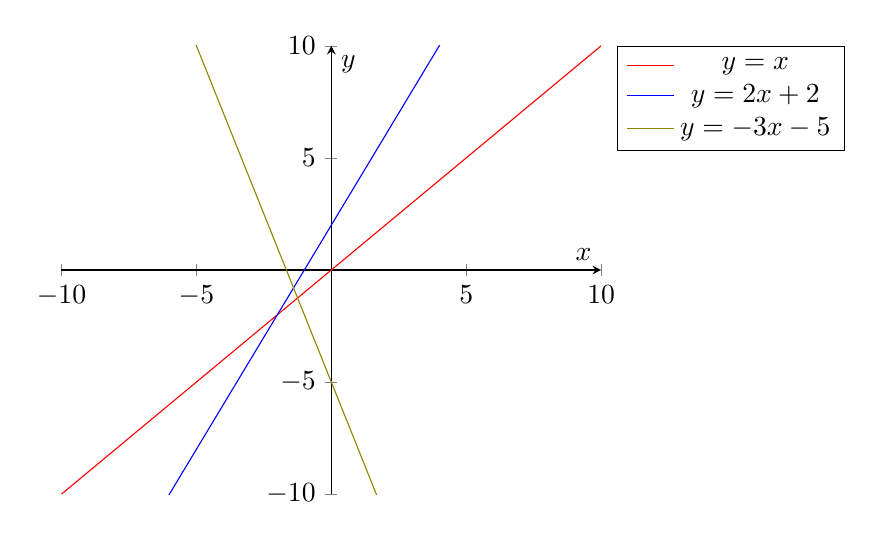
\begin{tikzpicture}
\begin{axis}[
    legend pos=outer north east,
    axis lines = left,
    axis x line = center,
    axis y line = center,
    xmin = -10,
    xmax = 10,
    ymin = -10,
    ymax = 10,
    xlabel = \(x\),
    ylabel = {\(y\)},
]
\addplot [
    domain=-10:10, 
    samples=100, 
    color=red,
]
{x};
\addlegendentry{\(y = x\)}
\addplot [
    domain=-10:10, 
    samples=100, 
    color=blue,
    ]
    {2*x + 2};
\addlegendentry{\(y = 2x + 2\)}
\addplot [
    domain=-10:10, 
    samples=100, 
    color=olive,
    ]
    {-3*x - 5};
\addlegendentry{\(y = -3x - 5\)}
\end{axis}
\end{tikzpicture}
\end{figure}

Here, $y = x$ meets the $y$ axis in the origin because $q$ is null, and it bisects perfectly the first and third quadrants of the cartesian plane because $m$ is equal to 1. The curves described by $y = 2x + 2$ and $y = -3x - 5$ are steeper (i.e., $y$ grows/decreases faster than $x$), because the absolute value of $m$ is greater than 1, and they meet the $y$ axis at 2 and -5 respectively. Moreover, $y = x$ and $y = 2x + 2$ are \textit{positive} linear functions because their slope is positive, i.e., $y$ values increase when $x$ values do, while the opposite holds for $y = -3x - 5$.\\
Since any flavor of Optimality Theory requires a conflict between constraints, and since \textsc{*Int Arg} is the one constraint to conflict with all the others in this account of object drop, Medina's model defines a linear function for the pairwise ordering of \textsc{*Int Arg} with respect to \textsc{Faith Arg} (\refeq{medinafunction_f}), \textsc{Telic End} (\refeq{medinafunction_t}), and \textsc{Perf Coda} (\refeq{medinafunction_p}), for a total of three different linear functions. In general, each function takes the form in \refeq{medinafunction_ex}, where the probability of \textsc{*Int Arg} being ranked above another constraint is $y$, $SPS_i$ is $x$, $\frac{\delta_k - \gamma_k}{SPS_{max} - SPS_{min}}$ is $m$, $\gamma_k - SPS_{min} (\frac{\delta_k - \gamma_k}{SPS_{max} - SPS_{min}})$ is $q$, and $\delta_k$ and $\gamma_k$ are, respectively, the values the function assumes at $SPS_{max}$ and $SPS_{min}$.

\begin{equation} \labeq{medinafunction_ex}
p(\textsc{*Int Arg} \gg \textrm{con}) = \frac{\delta_k - \gamma_k}{SPS_{max} - SPS_{min}} \cdot ({SPS_{i} - SPS_{min}}) + \gamma_k
\end{equation}

In particular, the three linear functions at play are the ones in \refeq{medinafunction_f}, \refeq{medinafunction_t}, and \refeq{medinafunction_p}.

\begin{equation} \labeq{medinafunction_f}
p(\textsc{*Int Arg} \gg \textsc{Faith Arg}) = \frac{\delta_1 - \gamma_1}{SPS_{max} - SPS_{min}} \cdot ({SPS_{i} - SPS_{min}}) + \gamma_1
\end{equation}

\begin{equation} \labeq{medinafunction_t}
p(\textsc{*Int Arg} \gg \textsc{Telic End}) = \frac{\delta_2 - \gamma_2}{SPS_{max} - SPS_{min}} \cdot ({SPS_{i} - SPS_{min}}) + \gamma_2
\end{equation}

\begin{equation} \labeq{medinafunction_p}
p(\textsc{*Int Arg} \gg \textsc{Perf Coda}) = \frac{\delta_3 - \gamma_3}{SPS_{max} - SPS_{min}} \cdot ({SPS_{i} - SPS_{min}}) + \gamma_3
\end{equation}

These functions take positive values in a range of possible values depending on the verbs' semantic selectivity. %Moreover, since the slope of each function results from the ratio between two positive-resulting differences (i.e., maximum minus minimum $y$ and $x$ values), the functions take values that are directly proportional to the verbs' Selectional Preference Strength.

\subsection{Logical step 2: relative probabilities of the 4 constraint re-rankings} \labsec{logicalmedina2}
At the beginning of this Section, it was observed that four constraints result in 24 possible re-ranking orders (listed in \reftab{medina_24rankings}), and that this large set of permutations actually reduces to just four possible re-rankings if one only cares for the relative position of \textsc{*Int Arg}. In fact, the model will favor an implicit object output whenever \textsc{*Int Arg} is ranked above all the relevant constraints, regardless of their order with respect to one another. A telic perfective input only results in an implicit object output when \textsc{*Int Arg} is ranked above the three other constraints, a telic imperfective input when \textsc{*Int Arg} is ranked above \textsc{Faith Arg} and \textsc{Telic End}, an atelic perfective input when \textsc{*Int Arg} is ranked above \textsc{Faith Arg} and \textsc{Perf Coda}, and an atelic imperfective input when \textsc{*Int Arg} is ranked above \textsc{Faith Arg} alone. This results in the four possible orderings in \reftab{medina_4rankings}.

% \begin{table}[htb] % the "htb" makes table env unfloaty
% \caption{Set of the four possible re-rankings of \textsc{*Int Arg} with respect to \textsc{Faith Arg}, \textsc{Telic End}, and \textsc{Perf Coda}, these being unordered with respect one to another.}
% \labtab{medina_4rankings} 
% \begin{tabular}{|l||c|c|c|c|}\hline 
%       & \vtop{\hbox{\strut \textbf{Telic}}\hbox{\strut \textbf{Perf}}}  &  \vtop{\hbox{\strut \textbf{Telic}}\hbox{\strut \textbf{Imperf}}} & \vtop{\hbox{\strut \textbf{Atelic}}\hbox{\strut \textbf{Perf}}} & \vtop{\hbox{\strut \textbf{Atelic}}\hbox{\strut \textbf{Imperf}}}\\
%       \hline\hline
% *I $\gg$ \{F, T, P\} & implicit  &  implicit   & implicit  & implicit \\ 
% P $\gg$ *I $\gg$ \{F, T\} & overt  &  implicit   & overt  & implicit \\
% T $\gg$ *I $\gg$ \{F, P\} & overt  &  overt   & implicit  & implicit \\
% \{T, P\} $\gg$ *I $\gg$ F & overt  &  overt   & overt  & implicit \\\hline
% \end{tabular}
% \end{table}

\begin{table}[htb] % the "htb" makes table env unfloaty
\caption{Set of the four possible re-rankings of \textsc{*Int Arg} with respect to \textsc{Faith Arg}, \textsc{Telic End}, and \textsc{Perf Coda}, these being unordered with respect one to another.}
\labtab{medina_4rankings} 
\begin{tabular}{l|cccc}
      & \vtop{\hbox{\strut \textbf{Telic}}\hbox{\strut \textbf{Perf}}}  &  \vtop{\hbox{\strut \textbf{Telic}}\hbox{\strut \textbf{Imperf}}} & \vtop{\hbox{\strut \textbf{Atelic}}\hbox{\strut \textbf{Perf}}} & \vtop{\hbox{\strut \textbf{Atelic}}\hbox{\strut \textbf{Imperf}}}\\
      \hline
*I $\gg$ \{F, T, P\} & implicit  &  implicit   & implicit  & implicit \\ 
P $\gg$ *I $\gg$ \{F, T\} & overt  &  implicit   & overt  & implicit \\
T $\gg$ *I $\gg$ \{F, P\} & overt  &  overt   & implicit  & implicit \\
\{T, P\} $\gg$ *I $\gg$ F & overt  &  overt   & overt  & implicit
\end{tabular}
\end{table}

The probability of each individual re-ranking ordering in \reftab{medina_4rankings} is equal to the joint probabilities of the independent pairwise orderings that comprise it. For instance, the probability of \textsc{*Int Arg} being ranked above all the other constraints is equal to the intersection (represented with $\cap$ in set theory) between the probability spaces of \textsc{*Int Arg} being ranked above \textsc{Faith Arg}, \textsc{*Int Arg} being ranked above \textsc{Telic End}, and \textsc{*Int Arg} being ranked above \textsc{Perf Coda}. This is rendered graphically in the Venn diagram in \reffig{venndiagram}, where the probability of \textsc{*Int Arg} being ranked above all the other constraints is colored in blue.

\begin{figure}[htb]
\caption{Graphical representation of the probability of \textsc{*Int Arg} being ranked above the three other constraints, in cyan in the Venn diagram.}
\labfig{venndiagram}
\begin{tikzpicture}
    \begin{scope}
    \clip \firstcircle;
    \clip \secondcircle;
    \fill[cyan] \thirdcircle;
    \end{scope}
\draw \firstcircle node[text=black,above] {$p(*I \gg F)$};
\draw \secondcircle node [text=black,below left] {$p(*I \gg T)$};
\draw \thirdcircle node [text=black,below right] {$p(*I \gg P)$};
    \end{tikzpicture}
    \end{figure}

In summary, the probabilities of the four rankings in \reftab{medina_4rankings} are computed as in \refeq{jointprobsmedina} to \refeq{jointprobsmedina4}. Whenever an equation features the subtraction of the probability of an event from 1, it means that the computation is taking into account the cases when that event is \textit{not} happening, given that probabilities can vary between 0 (impossible event) and 1 (certain event). For instance, since in \refeq{jointprobsmedina2} \textsc{Faith Arg} ranks above \textsc{*Int Arg}, the partial probability included in the computation is [1 - p(\textsc{*Int Arg} $\gg$ \textsc{Faith Arg})], namely the probability of \textsc{*Int Arg} \textit{not} being ranked above \textsc{Faith Arg}. \labpage{jointprobz}

\begin{align}  \labeq{jointprobsmedina} % https://tex.stackexchange.com/questions/332430/correctly-left-align-a-set-of-equations
    & p(*I \gg {F, T, P}) = p(*I \gg F) \cdot p(*I \gg T) \cdot p(*I \gg P) \\
    & p(P \gg *I \gg {F, T}) = p(*I \gg F) \cdot p(*I \gg T) \cdot [1 - p(*I \gg P)] \labeq{jointprobsmedina2}\\
    & p(T \gg *I \gg {F, P}) = p(*I \gg F) \cdot [1 - p(*I \gg T)] \cdot p(*I \gg P) \labeq{jointprobsmedina3}\\
    & p({T, P} \gg *I \gg F) = p(*I \gg F) \cdot [1 - p(*I \gg T)] \cdot [1 - p(*I \gg P)] \labeq{jointprobsmedina4}
\end{align}

\subsection{Logical step 3: grammaticality of implicit object output as sum of probabilities for each aspectual type} \labsec{logicalmedina3}
Returning to \reftab{medina_4rankings}, the next step consists in determining the probability of an implicit object output for each of the four aspectual features in the input (the columns of the table). It is possible to achieve this result by summing the probabilities of the individual partial orderings where \textsc{*Int Arg} is ranked above the relevant constraints (the rows of the table). Thus, the likelihood of the object being dropped for each aspectual type is computed as in \refeq{aspectualprobs} to \refeq{aspectualprobs4}.

\begin{align}  \labeq{aspectualprobs}
    & p(\text{implicit})\textsubscript{Telic Perfective} = p(*I \gg {F, T, P}) \\
    & p(\text{implicit})\textsubscript{Telic Imperfective} = p(*I \gg {F, T, P}) + p(P \gg *I \gg {F, T}) \labeq{aspectualprobs2}\\
    & p(\text{implicit})\textsubscript{Atelic Perfective} = p(*I \gg {F, T, P}) + p(T \gg *I \gg {F, P}) \labeq{aspectualprobs3}\\
    & p(\text{implicit})\textsubscript{Atelic Imperfective} = p(*I \gg {F, T, P}) + p(T \gg *I \gg {F, P}) + \nonumber \\ & + p(P \gg *I \gg {F, T}) + p({T, P} \gg *I \gg F) \labeq{aspectualprobs4}
\end{align}

As stated at the beginning of this Section, in the stochastic model of the implicit object construction by \textcite{Medina2007} these probabilities indicate the gradient grammaticality of indefinite object drop for each aspectual type of input.\\
Atelic imperfective inputs violate a proper subset of the constraints violated by other aspectual types of input. Hence, also considering \reftab{medina_4rankings} and the probabilities \refeq{aspectualprobs} to \refeq{aspectualprobs4}, it is evident that the implicit object output is most likely to be grammatical with atelic imperfective inputs. Following this line of reasoning, it results that telic perfective inputs have the lowest probability to yield an implicit object output, and that the likelihood of atelic perfective and telic imperfective inputs to allow for the object to be dropped is intermediate. The relative object-dropping probability of atelic perfective inputs with respect to telic imperfective inputs depends on the parameters of the functions in \refeq{medinafunction_f}, \refeq{medinafunction_t}, and \refeq{medinafunction_p}. This state of affairs is depicted in \reffig{mock_scatter_medina}, an adaptation of the graph provided by \textcite[108]{Medina2007}.

\begin{figure}[htb]
\caption{Hypothetical representation of the relationship between semantic selectivity and the probability (as a proxy to grammaticality) of an implicit object output in the stochastic model by \textcite{Medina2007}. }
\labfig{mock_scatter_medina}
  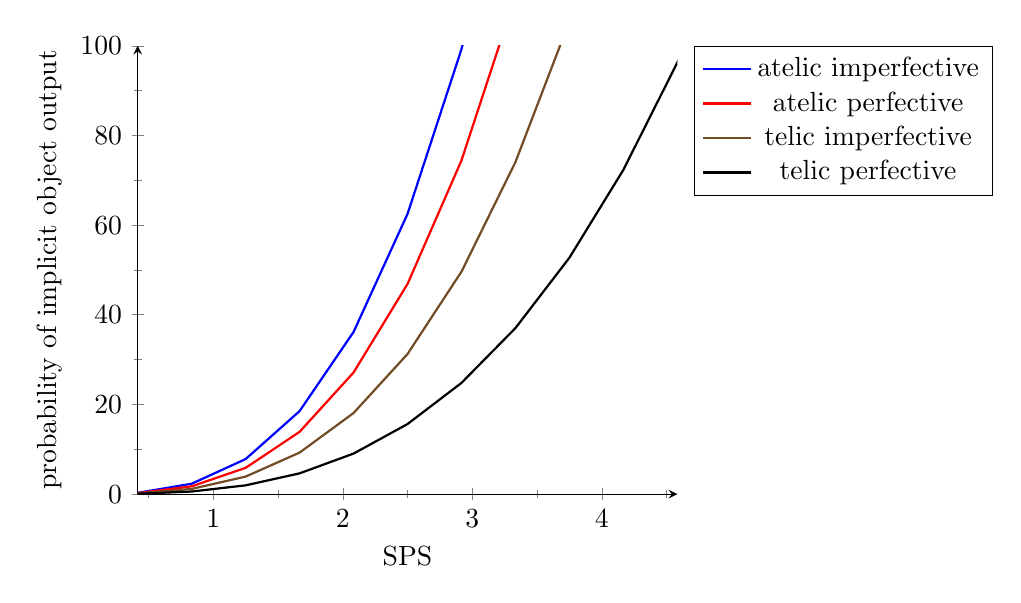
\begin{tikzpicture}
\begin{axis}[legend pos=outer north east,
    axis lines = left,scaled ticks=false,ymax=100,ymin=0,minor tick num=1,xlabel={SPS}, ylabel={probability of implicit object output}]
      \addplot+[no marks,thick] {4*(x^3)};
      \addlegendentry{atelic imperfective};
      \addplot+[no marks,thick] {3*(x^3)};
      \addlegendentry{atelic perfective};
      \addplot+[no marks,thick] {2*(x^3)};
      \addlegendentry{telic imperfective};
      \addplot+[no marks,thick] {x^3};
      \addlegendentry{telic perfective};
    \end{axis}
  \end{tikzpicture}
\end{figure}

The curves in \reffig{mock_scatter_medina} are cubic functions because the computations in \refeq{jointprobsmedina} to \refeq{jointprobsmedina4} involve the multiplication of the three linear functions of the type illustrated in \refeq{medinafunction_ex}. This means that the unknown $SPS_i$ (the $x$ of the linear function) gets multiplied three times by itself, resulting in ${SPS_i}^3$, which yields a cubic curve. Of course, all the parameters in the complex function in \refeq{medinafunction_ex} are part of the newly created cubic function, but they do not result in a higher grade (i.e., more than cubic) polynomial function since they are not unknowns of the function.

\section{Implementing a probabilistic constraint ranking} \labsec{medinacomputation}

\subsection{Introduction} \labsec{3stepcompmedina}
The three-step logic illustrated in \refsec{rankingmedina} is mirrored by the three-step procedure used to computationally implement the probabilistic constraint ranking. The computational steps devised by Medina are as follows: \labpage{3stepcompmedina}

\begin{enumerate}
    \item the grammaticality of the indefinite object drop is quantified via an acceptability judgment survey, the results thereof are equated to the probability of an implicit object output for a given input;
    \item the probability of each of the four possible constraint orderings can be estimated via the probability of an implicit object output;
    \item knowing the probability of each constraint ordering, it is possible to estimate the probability of \textsc{*Int Arg} dominating each constraint.
\end{enumerate}

As is evident from comparing the logical and the computational steps (see \reftab{medina_nicetable}), the technical implementation of the model goes backwards with respect to the underlying logic.

\begin{table}[htb] % the "htb" makes table env unfloaty
\caption{Three-step design of Medina's model, where the computational steps mirror the logical steps.}
\labtab{medina_nicetable} 
\begin{tabular}{c c}
 & \\
\cmidrule{1-1} % richiede un range! else esce COMPILE TIMEOUT ERROR
\textbf{Logic} &                      \\
\textbf{$\downarrow$} &                      \\ \hline
step 1         & step 3               \\
step 2         & step 2               \\
step 3         & step 1               \\ \hline
               & \textbf{$\uparrow$} \\
               & \textbf{Computation} \\
\cmidrule{2-2}           
\end{tabular}
\end{table}

Let us discuss each computational step in more detail.

\subsection{Computational step 1: Collecting acceptability judgments} The collection of acceptability judgments is not a part of the computational procedure \textit{per se}, unlike the estimation of the parameters of the linear functions. However, since acceptability judgments are directly equated to the probability of an implicit object output, the fine points of their collection belong to this Section nonetheless. I will now present the main aspects of Medina's experimental design, which the interested reader can integrate with additional information by \textcite[110-134]{Medina2007}.\\
The linguistic predictors of object drop under consideration are semantic selectivity, telicity, and perfectivity. Among these, semantic selectivity and telicity\sidenote{Based on \textcite{Olsen1997} and pertaining observations throughout this chapter. Refer to \refsec{telicity} for more details.} are inherent properties of each verb, while perfectivity is a sentence-level property. For this reason, the verbs in Medina's experiment are annotated with respect to their semantic selectivity and telicity, while sentences are manipulated for perfectivity. This results in a 2x2 factorial design\sidenote{An experimental design with two independent variables having two levels each, resulting in four experimental conditions.} where each verb, having its own selectivity and telicity profile, appears both with and without a direct object, both having and lacking the perfectivity feature. The examples in \ref{medina_exstim} are adapted from \textcite[113]{Medina2007}.

\ex. \label{medina_exstim} \a. \label{medina_exstim1} Michael had brought.
\b. \label{medina_exstim2}  Michael was bringing.
\c. \label{medina_exstim3}  Sarah had brought a gift.
\d. \label{medina_exstim4}  Sarah was bringing a gift.

The telicity of each verb was deemed to be [+Telic] if two out of three tests yielded a telic interpretation, [-Telic] otherwise. As discussed in \refsec{predictor_telicity} in regards to the telicity tests of choice in my own model, there is something to be said about the feasibility of this particular set of tests. However, they yielded very consistent results, and henceforth they cannot be considered as a crack in the otherwise solid foundation of Medina's design. The three tests used by \textcite[302-303]{Medina2007}, first introduced in \refsec{medinatelicity}, are as follows.
\begin{itemize}
    \item \textbf{The \textit{almost} test.} Predicates marked as [+telic] and appearing with the adverb \textit{almost} (e.g., \textit{Tony almost packed}) can be interpreted as describing either an event that has begun but has not finished, or an event that has not yet begun. On the contrary, [-telic] predicates with \textit{almost} (e.g., \textit{Tony almost ate}) can only get the second interpretation.
    \item \textbf{The \textit{in/for} test.} [+telic] predicates are more natural with \textit{in X time} as an adjunct (e.g., \textit{Michelle made some stuff in/*for five minutes}), while [-telic] ones prefer \textit{for X time} (e.g., \textit{Michelle read *in/for five minutes}).
    \item \textbf{The \textit{counting} test.} Counting a [+telic] predicate results in a natural interpretation where it denotes multiple, separate events (e.g., \textit{Edgar opened some stuff three times}), while counted [-telic] predicates appear as if denoting multiple instances of the same event (e.g., \textit{Edgar watched some stuff three times}).
\end{itemize}

Using a set of 30 transitive verbs of interest and 10 intransitive verbs resulted in a set of 160 sentences to be used as experimental stimuli (because of Medina's 2x2 design). The 30 transitive verbs were the same used by \textcite{Resnik1993, Resnik1996} to test his Selectional Preference Strength, since \textcite{Medina2007} employs the same measure to quantify semantic selectivity. Of the 160 stimuli, the 40 intransitive sentences resulting from the 10 intransitive non-target verbs were used as fillers to distract the participants from the real focus of the experiment, the 60 transitive sentences with an overt object were used as controls (since they had to be grammatical by default), and the remaining 60 sentences featuring a transitive verb used \textit{without} a direct object were the actual target of the experiment.\\
A total of 15 native speakers of English were recruited as participants among the undergraduate students of Johns Hopkins University and rewarded class credit for their effort. Each of them saw all the stimuli in every experimental condition in randomized order, i.e., the experiment followed a within-subject crossed design. Participants partook in a short training session with 3 mock stimuli before accessing the experiment proper, and received immediate feedback. Both in the training session and the experimental session, participants had to score each stimulus on a 5-point Likert scale ranging from 1 (ungrammatical) to 5 (fully grammatical).

\subsection{Computational step 2: Judgments and probabilities} The acceptability judgments thus obtained for each verb in each experimental condition were considered equal to the probability of the implicit object output to be returned by the stochastic model based on all the possible re-rankings of the constraints at play for that given input. The judgment scores were then used to estimate the probabilities of the four possible constraint rankings in \reftab{medina_4rankings}, which in turn were used to estimate the probabilities of \textsc{*Int Arg} dominating each of the other three constraints. Let us retrace the computational steps that lead to this result.\\
As shown in \refsec{logicalmedina3}, the probability of an implicit object output for each aspectual type of input is equal to the sum of the probabilities of the individual partial orderings where \textsc{*Int Arg} is ranked above the relevant constraints. This is shown in \refeq{aspectualprobs} to \refeq{aspectualprobs4}, reported here again for ease of consultation. % joint probability of the independent pairwise rankings of the relevant constraints ERA SBAGLIATO

\begin{align*}  \tag{\refeq{aspectualprobs}}
    & p(\text{implicit})\textsubscript{Telic Perfective} = p(*I \gg {F, T, P}) \\
    & p(\text{implicit})\textsubscript{Telic Imperfective} = p(*I \gg {F, T, P}) + p(P \gg *I \gg {F, T}) \tag{\refeq{aspectualprobs2}}\\
    & p(\text{implicit})\textsubscript{Atelic Perfective} = p(*I \gg {F, T, P}) + p(T \gg *I \gg {F, P}) \tag{\refeq{aspectualprobs3}}\\
    & p(\text{implicit})\textsubscript{Atelic Imperfective} = p(*I \gg {F, T, P}) + p(T \gg *I \gg {F, P}) + \nonumber \\ & + p(P \gg *I \gg {F, T}) + p({T, P} \gg *I \gg F) \tag{\refeq{aspectualprobs4}}
\end{align*}

Based on the calculations in \refeq{jointprobsmedina} to \refeq{jointprobsmedina4}, the aforementioned sums of probabilities can be computed as follows in \refeq{jointcomplete} to \refeq{jointcomplete4}, where the probability of \textsc{*Int Arg} outranking \textit{all} the relevant constraints is equal to the joint probability of the independent pairwise rankings of \textit{each} constraint with respect to \textsc{*Int Arg} (as explained in \refsec{logicalmedina2}).

\begin{align}  \labeq{jointcomplete}
    & p(\text{implicit})\textsubscript{Telic Perfective} = p(*I \gg F) \cdot p(*I \gg T) \cdot p(*I \gg P) \\
    & p(\text{implicit})\textsubscript{Telic Imperfective} = p(*I \gg F) \cdot p(*I \gg T) \cdot p(*I \gg P) + \nonumber \\ & + p(*I \gg F) \cdot p(*I \gg T) \cdot [1 - p(*I \gg P)] \labeq{jointcomplete2}\\
    & p(\text{implicit})\textsubscript{Atelic Perfective} = p(*I \gg F) \cdot p(*I \gg T) \cdot p(*I \gg P) + \nonumber \\ & + p(*I \gg F) \cdot [1 - p(*I \gg T)] \cdot p(*I \gg P) \labeq{jointcomplete3}\\
    & p(\text{implicit})\textsubscript{Atelic Imperfective} = p(*I \gg F) \cdot p(*I \gg T) \cdot p(*I \gg P) + \nonumber \\ & + p(*I \gg F) \cdot [1 - p(*I \gg T)] \cdot p(*I \gg P) + \nonumber \\ & + p(*I \gg F) \cdot p(*I \gg T) \cdot [1 - p(*I \gg P)] + \nonumber \\ & + p(*I \gg F) \cdot [1 - p(*I \gg T)] \cdot [1 - p(*I \gg P)] \labeq{jointcomplete4}
\end{align}

\subsection{Computational step 3: Parameter estimation} The last step involves \refeq{medinafunction_f}, \refeq{medinafunction_t}, and \refeq{medinafunction_p}, where the ranking of \textsc{*Int Arg} with respect to the other three constraints was defined as a (linear) function of the input verb's semantic selectivity. Plugging them in \refeq{jointcomplete} results in the (cubic) function in \refeq{cubic_telperf}, describing the probability of an implicit object output with a telic perfective input depending on the specific verb's semantic selectivity.

\begin{align}  \labeq{cubic_telperf}
    & p(\text{implicit})\textsubscript{Telic Perfective} = [\frac{\delta_1 - \gamma_1}{SPS_{max} - SPS_{min}} \cdot ({SPS_{i} - SPS_{min}}) + \gamma_1] \cdot \nonumber \\ & \cdot [\frac{\delta_2 - \gamma_2}{SPS_{max} - SPS_{min}} \cdot ({SPS_{i} - SPS_{min}}) + \gamma_2] \cdot \nonumber \\ & \cdot [\frac{\delta_3 - \gamma_3}{SPS_{max} - SPS_{min}} \cdot ({SPS_{i} - SPS_{min}}) + \gamma_3]
\end{align}

The value of the function, i.e., $p(\text{implicit})\textsubscript{Telic Perfective}$, is the average acceptability judgment for a telic perfective input with a known SPS, i.e., $SPS_{i}$ in the equation. The values of $SPS_{max}$ and $SPS_{min}$ are known, since they are the maximum and minimum Selectional Preference Strength values in Resnik's list, respectively. Henceforth, the equation has only to be solved for $\delta_i$ and $\gamma_i$, which are the values the function takes at $SPS_{max}$ and $SPS_{min}$ respectively. A similar reasoning applies to telic imperfective, atelic perfective, and atelic imperfective inputs, once again plugging \refeq{medinafunction_f}, \refeq{medinafunction_t}, and \refeq{medinafunction_p} into \refeq{jointcomplete2}, \refeq{jointcomplete3}, and \refeq{jointcomplete4}.\\
At the end of this process, the experimenter is left with a set of $n$ equations, each having six unknowns to be solved for, where $n$ is the total number of target sentences among the stimuli. In order to calculate $\delta_i$ and $\gamma_i$, the judgments (i.e., the probabilities of object drop which serve as values of the functions) underwent two preprocessing steps in Medina's pipeline, namely:
\begin{enumerate}
    \item for each target sentence, the 15 judgments provided by 15 participants were averaged into a single numerical value, and
    \item this numerical value was converted linearly to fall between 0 and 1, since this is the proper range for probabilities.
\end{enumerate}

Medina estimated the values of the unknown parameters using Excel Solver\sidenote{An add-in component of Microsoft Excel used to find the optimal value of a function based on several constraints.}, based on the following two constraints: \labpage{medinaexcelsolver}
\begin{itemize}
    \item $\delta_i$ and $\gamma_i$ have to fall between 0 and 1;
    \item the sum-squared error between the predictions of the model and the actual grammaticality judgment data have to be minimized.
\end{itemize}
Thanks to these constraints, the model outputs predicted grammaticality values in the 0-1 probability range.

\subsection{Summary of results} \labsec{medinaresults}
The values of $\delta_i$ and $\gamma_i$ Medina found as a result of this optimization indicate that, in English, \textsc{*Int Arg} is more likely to dominate each of the other three constraints when the verb is highly semantically selective, and this is most evident for \textsc{Telic End}. The actual values computed by the model are in \reftab{medina_deltagammas}.

\begin{table}[htb] % the "htb" makes table env unfloaty
\caption{Values of unknown parameters $\delta_i$ and $\gamma_i$ as computed in Medina's stochastic model.}
\labtab{medina_deltagammas} 
\begin{tabular}{l|cc}
                                                                                & $\gamma$ & $\delta$ \\
                                                                                \hline
p(\textsc{*Int Arg} $\gg$ \textsc{Faith Arg}) & 0.70        & 0.82        \\
p(\textsc{*Int Arg} $\gg$ \textsc{Telic End}) & 0.36        & 1.00        \\
p(\textsc{*Int Arg} $\gg$ \textsc{Perf Coda}) & 0.65        & 0.80       
\end{tabular}
\end{table}

These results are visualized in \reffig{medina_intargabove}, adapted from the figures in \textcite[143-144]{Medina2007}.

\begin{figure}[htb]
\caption{Graphical representation of the values of $\gamma$ and $\delta$ in Medina's model.}
\labfig{medina_intargabove}
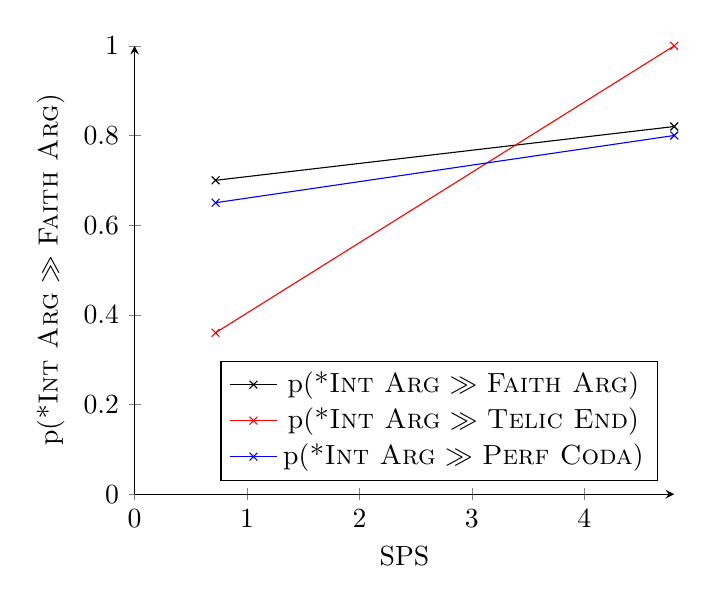
\begin{tikzpicture}
    \begin{axis}[legend pos=south east, xmin=0, ymin=0, ymax=1, axis lines = left,scaled ticks=false, xlabel={SPS}, ylabel={p(\textsc{*Int Arg} $\gg$ \textsc{Faith Arg})}] 
        \addplot[color=black,mark=x] coordinates {
        (0.72,0.70) 
        (4.80,0.82) 
    }; 
      \addlegendentry{p(\textsc{*Int Arg} $\gg$ \textsc{Faith Arg})};
            \addplot[color=red,mark=x] coordinates {
        (0.72,0.36) 
        (4.80,1.00) 
    }; 
    \addlegendentry{p(\textsc{*Int Arg} $\gg$ \textsc{Telic End})};
            \addplot[color=blue,mark=x] coordinates {
        (0.72,0.65) 
        (4.80,0.80) 
    }; 
    \addlegendentry{p(\textsc{*Int Arg} $\gg$ \textsc{Perf Coda})};
    % \node [above] at (axis cs:  0.72,0.70) {(0.72,0.70)};
    % \node [above left] at (axis cs:  4.80,0.82) {(4.80,0.82)};
    \end{axis} 
\end{tikzpicture}
\end{figure}

Knowing the actual values of these parameters, it is possible to plug them into \refeq{cubic_telperf} (and the equivalent functions for the three other aspectual types of input) to let the model predict the grammaticality of an implicit object output in terms of its probability as a function of semantic selectivity. Graphically, the state of affairs that was hypothesized in \reffig{mock_scatter_medina} looks like in \reffig{medina_predictedresults} (adapted from \textcite[145]{Medina2007}) in Medina's model of indefinite object drop in English. The figure shows the probability of an implicit object output for all possible aspectual types depending on SPS values ranging from 0 to 5, based on the $\gamma$ and $\delta$ values estimated in the model (shown in \reftab{medina_deltagammas}).

\begin{figure}[htb]
\caption{Realistic representation of the relationship between semantic selectivity and the probability (as a proxy to grammaticality) of an implicit object output in Medina's model, based on computed $\gamma$ and $\delta$ values.}
\labfig{medina_predictedresults}
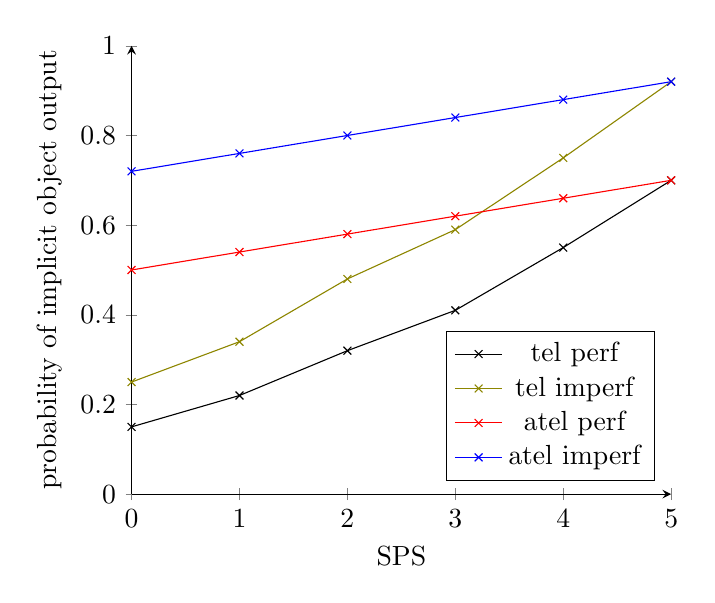
\begin{tikzpicture}
    \begin{axis}[legend pos=south east, xmin=0, ymin=0, ymax=1, axis lines = left,scaled ticks=false, xlabel={SPS}, ylabel={probability of implicit object output}] 
        \addplot[color=black,mark=x] coordinates {
        (0,0.15) 
        (1,0.22) 
        (2,0.32) 
        (3,0.41) 
        (4,0.55) 
        (5,0.70) 
    }; 
      \addlegendentry{tel perf};
        \addplot[color=olive,mark=x] coordinates {
        (0,0.25) 
        (1,0.34) 
        (2,0.48) 
        (3,0.59) 
        (4,0.75) 
        (5,0.92) 
    }; 
      \addlegendentry{tel imperf};  
        \addplot[color=red,mark=x] coordinates {
        (0,0.50) 
        (1,0.54) 
        (2,0.58) 
        (3,0.62) 
        (4,0.66) 
        (5,0.70) 
    }; 
      \addlegendentry{atel perf};    
        \addplot[color=blue,mark=x] coordinates {
        (0,0.72) 
        (1,0.76) 
        (2,0.80) 
        (3,0.84) 
        (4,0.88) 
        (5,0.92) 
    }; 
      \addlegendentry{atel imperf};        
    \end{axis} 
\end{tikzpicture}
\end{figure}

Finally, it results that:
\begin{itemize}
    \item the probability of an implicit object output is directly proportional to the verb's SPS for all aspectual types of input;
    \item the relative probabilities hypothesized in \reffig{mock_scatter_medina} are also shown in the actual results, with the implicit object construction being most likely with atelic imperfective inputs and least likely with telic perfective inputs;
    \item due to semantic selectivity, there is an interaction between aspectual features so that telic imperfective inputs are less likely to accept object drop than atelic perfective inputs when the verb's SPS is low (approximately lower than 3 in Resnik's and Medina's case), while the opposite happens for verbs with a higher SPS;
    \item in \reffig{medina_predictedresults}, the curves for inputs having the same telicity feature are more-or-less parallel because of the strong telicity effect shown in the steep p(\textsc{*Int Arg} $\gg$ \textsc{Telic End}) curve in \reffig{medina_intargabove}, where it is also easy to spot the interaction between telicity and perfectivity that was mentioned in the previous bullet point.
\end{itemize}

In \refch{predictors}, I will open the experimental part of this thesis by presenting the five predictors I included in my own Stochastic Optimality Theoretic model of the implicit indefinite object construction in English and Italian.